\section{Differentialgleichungen}
\[ F(x,y,y',\dots,y^{(n)}) = 0 \]
\textbf{Autonom:} $y' = f(x) \qquad \rightarrow$ nur von $y$ abhängig.\\
\textbf{Explizit:} explizit falls nach $y^{(n)}$ aufgelöst werden kann, ansonsten implizit

\subsection{Lineare homogene autonome DGL 1. Ordnung}

\[ \dfrac{d}{dt}y(t)+ay(t)=0 \qquad y(t_0)=y_0 \]
\begin{tabular}{ll}
Ansatz: & $y(t) = e^{\lambda t}$\\
Einsetzen in DGL: & $\lambda e^{\lambda t} + ae^{\lambda t} = 0$\\
Charakteristisches Polynom: & $\lambda = -a$\\
Allgemeine Lösung: & $y(t) = Ce^{-ax}$\\
\multicolumn{2}{l}{Freiheitsgrad $C$ mit Anfangswert bestimmen} \\
\end{tabular}

\subsection{Lösungsformeln 1. Ordnung}
\subsubsection{Lineare DGL}
\begin{tabular}{p{6cm}p{2cm}p{0.2cm}p{3.8cm}p{6.5cm}}
\textbf{Form:} \quad $y'(x) = f(x) \cdot y(x) + g(x)$ &
\textbf{Vorgehen:} &
1. & $\mu(t)$ berechnen: & $\mu(t) = e^{\int p(t) dt}$ \\ &&
2. & L"osung: & $y(t) = \frac{1}{\mu(t)} \cdot ( \int \mu(t) g(t) dt +c)$ \\ &&
\end{tabular}
Lösung existiert und eindeutig falls $p(t)$ und $g(t)$ stetig.\\
\textbf{Bsp}: $t^3 \cdot y'(t) + 4 t^2 \cdot y(t) = e^{-t} \quad \Longrightarrow \quad y'(t) + \underbrace{4 \frac{1}{t}}_{p(t)} \cdot y(t) = \underbrace{\frac{1}{t^3} e^-t}_{g(t))}$

\subsubsection{Separierbare DGL (wenn autonom, dann auch separierbar)}
\begin{tabular}{p{6cm}p{2cm}p{0.2cm}p{6cm}p{6.5cm}}
\textbf{Form:} \quad $y'(x) = g(x) \cdot h(y)$ &
\textbf{Vorgehen:} &
1.& Gleichung umschreiben: & $\frac{dy}{dx} = g(x) \cdot h(y)$\\ &&
2.& alle $x$-Terme auf die linke Seite: & $\frac{1}{h(y)}dy = g(x) dx$ \\ &&
3.& beide Seiten integrieren: & $\int \frac{1}{h(y)}dy = \int g(x)dx$ \\ & & & & C folgt aus Anf. Bed.\\
\end{tabular} \\
\textbf{Bsp}: $y' = -\frac{x}{y} \Rightarrow \frac{dy}{dx} = -\frac{x}{y} \Rightarrow ydy = -xdx \Rightarrow \int ydy = - \int xdx \Rightarrow \frac{1}{2}y^2 = -\frac{1}{2} x^2 + C$

\subsubsection{Exakte DGL}
\begin{tabular}{p{6.5cm}p{2cm}p{0.2cm}p{3.8cm}p{6.5cm}}
\textbf{Form:} \quad $M(x,y) + N(x,y)\cdot y'(x) = 0$ &
\textbf{Vorgehen:} &
1. & Kompatibilit"ats Bed. pr"ufen: & $\diffp{M(x,y)}{y} = \diffp{N(x,y)}{x}$ \\ &&
2. & $ M(x,y) = \dfrac{d}{dx}\Psi(x,y)$ & $N(x,y) = \dfrac{d}{dy}\Psi(x,y) $ \\ &&
3. & $Q(x,y)$ berechnen: & $Q(x,y) = \int M(x,y) dx$ \\ &&
4. & $\diffp{h(y)}{y}$ berechnen: & $\diffp{h(y)}{y} = N(x,y) - \diffp{Q(x,y)}{y}$ \\ &&
5. & $h(y)$ berechnen: & $h(y) = \int \diffp{h(y)}{y} dy $ \\ &&
6. & L"osung: & $\Psi(x,y) = Q(x,y) + h(y) = c $ \\
\end{tabular} \\
\textbf{Bsp}: $(9x^2 + y -1)dx - (4y -x)dy = 0 \quad \Longrightarrow \quad  \underbrace{9x^2 +y -1}_{M(x,y)} + \underbrace{(-(4y -x))}_{N(x,y)} \cdot \diffp{y}{x} = 0$

\subsubsection{Lösbarkeit}
Eine DGL ist dann lösbar, wenn
\begin{itemize}
	\item 1. Ordnung (DGL oder DGL-System)
	\item eindeutig wenn Anfangswerte gegeben sind
	\item Lipschitz-Stetigkeit erfüllt ist: $\lvert f(t,x_1) - f(t,x_2)\rvert \leq L \lvert x_1 - x_2 \rvert, L = const.$, welche nicht von $y$ abhängt.
\end{itemize}

\subsubsection{Substitution}
\begin{tabular}{p{4cm}p{6cm}}
	$y' = f(ax + by + c)$ & Substitution mit $z = ax + by + c$\\
	& $z = \frac{x}{y}$ und $y' = xz' + z$ \\
\end{tabular}

\subsection{Lineare homogene Differentialgleichung 2. Ordnung}
\begin{tabular}{ll}
	DGL:                       & $a \cdot y''(t) + b \cdot y'(t) + c \cdot y(t) = 0$                                                     \\
	Ansatz:                    & $y(t) = e^{\lambda t}$                                                                                  \\
	Einsetzen in DGL           & $\rightarrow$ Charakteristisches Polynom: $a\lambda^2 + b\lambda +c =0$                                 \\
	Nullstellen der Gleichung: & $\lambda_1,\lambda_2 = \frac{-b \pm \sqrt{b^2 - 4ac}}{2a}$                                              \\
	Fall 1:                    & $\lambda_1,\lambda_2 =$ reell $\rightarrow y_1(t) = e^{\lambda_1 t}, y_2(t) = e^{\lambda_2 t}$          \\
	Fall 2:                    & $\lambda = \lambda_1 = \lambda_2 =$ reell $\rightarrow y_1(t) = e^{\lambda t}, y_2(t) = te^{\lambda t}$ \\
	Fall 3:                    & $\lambda_1,\lambda_2* =$ komplex $\rightarrow z_1(t) = e^{\lambda_1 t}, z_2(t) = e^{\lambda_2 t} $       \\
	                           & $y_1(t) = Real(z_1)$ und $y_2(t) = Imag(z_1)$                                                           \\
	                           & oder: $a \pm j\beta: e^{ax}\cos(\beta x), e^{ax} \sin(\beta x)$\\
	Allgemeine Lösung:         & $y(t) = C_1y_1(t) + C_2y_2(t)$                                                                          \\
	Freiheitsgrade:            & $C_1,C_2$ mit Hilfe der gegebenen Anfangsbedingungen bestimmen.
\end{tabular} \\ \\
$\Rightarrow$ wenn \textbf{$n.$ Ordnung} immer noch ein $\cdot t$ mehr (wie im 2. Fall).\\ 

\subsection{Inhomogen 2. Ordnung}
\begin{tabbing}
1. Homogenes System lösen \= $a \cdot y''(t) + b \cdot y'(t) + c \cdot y(t) = 0$\\
2. Inhomogener Ansatz \> $a \cdot y''(t) + b \cdot y'(t) + c \cdot y(t) = g(t)$\\
\>\begin{tabular}{|l|l|}
	\hline
	\textbf{Störfunktion $g(x)$} & \textbf{Zugehöriger Ansatz für $y_s(x)$} \\ \hline
	$a$ (const)					 & $b$ (const) \\ \hline
	$a_0 + a_1x + \dots + a_mx^m$& $b_0 + b_1x+ \dots  b_mx^m$ \\ \hline
	$ae^{\lambda x}$			 & $be^{\lambda x}$ \\ \hline
	$a \sin(mx)$ & \\ 
	$b \cos(mx)$				 & $c \sin(mx) + d \cos(mx)$ \\
	$a \sin(mx) + b \cos(mx)$ & \\ \hline
\end{tabular}\\ \\
3. $y_s(x)$ in DGL einsetzen. \\
4. Zusammensetzen \> $y(t)=y_h(t)+y_p(t)$
\end{tabbing}
\subsection{Variation der Konstanten}
Hat man eine lineare, inhomogene Differentialgleichung 2. Ordnung mit folgender Struktur:\\
\begin{equation*}
y''(t) + p(t)y'(t) + q(t)y(t) = g(t)
\end{equation*}

Um die Variation der Konstanten verwenden zu  können, muss das System in ein System 1. Ordnung gebracht werden:\\
\begin{equation*}
x'(t) = A(t)x(t) + b(t)
\end{equation*}
\begin{equation*}
	\begin{vmatrix} 
	        y'(t)\\ 
	        y''(t)\\   
	\end{vmatrix}
	=
	\begin{vmatrix} 
	        x_1'(t)\\ 
	        x_2'(t)\\   
	\end{vmatrix}
	=
	\begin{vmatrix} 
	        0 && 1\\ 
	       -q(t) && -p(t)\\   
	\end{vmatrix}
	\begin{vmatrix} 
	        x_1(t)\\ 
	        x_2(t)\\   
	\end{vmatrix}
	+
	\begin{vmatrix} 
	        0\\ 
	        g(t)\\   
	\end{vmatrix}
\end{equation*}
In einem ersten Schritt wird die homogene Gleichung gelöst und wir erhalten zwei Fundementallösungen $y_1(t)$ und $y_2(t)$, damit erhalten wir eine Fundamentalmatrix der Form: \\
\begin{equation*}
X(t) = 
	\begin{vmatrix} 
	        y_1(t) && y_2(t)\\ 
	        y_1'(t) && y_2'(t)\\ 
	\end{vmatrix}
\end{equation*}
Um nun die partikuläre Lösung zu erhalten, verwenden wir folgende Gleichung: 
\begin{equation*}
y_P(t) = X(t) \int{X(t)^{-1}b(t)dt}
\end{equation*}
Die gesamte Lösung ergibt sich dann wieder aus der Summe der homogenen sowie der partikulären Lösung. 

\subsubsection{Richtungsfeld und Lösung - Begriff der Lösung}
Die Lösung der Differentialgleichung $\frac{d}{dt}x(t) = f(t,x(t))$ ist eine parametrisierte Kurve x(t). Die Ableitung nach t ist demnach der Tangentenvektor an diese Kurve. Die Diffgleichung enthält demnach die Information über die Tangentenvektoren an ihre Lösungskurven. 
Das bedeutet, auch ohne die Lösung können wir die rechte Seite der Gleichung - d.h. die Tangentenvektoren - zeichnen. Das Lösen der Gleichung ist schlussendlich nur das Einpassen von Kurven in dieses Vektorfeld. Solche Kurven sind die Trajektorien der Gleichung. Die Trajektorie ist jedoch \textbf{nicht} die Lösung, da als Beispiel die Zeitkomponente fehlt. Hätte man (t,x(t)), hätte man die gesamte Lösung. 
\begin{minipage}[h]{0.35\textwidth} 
	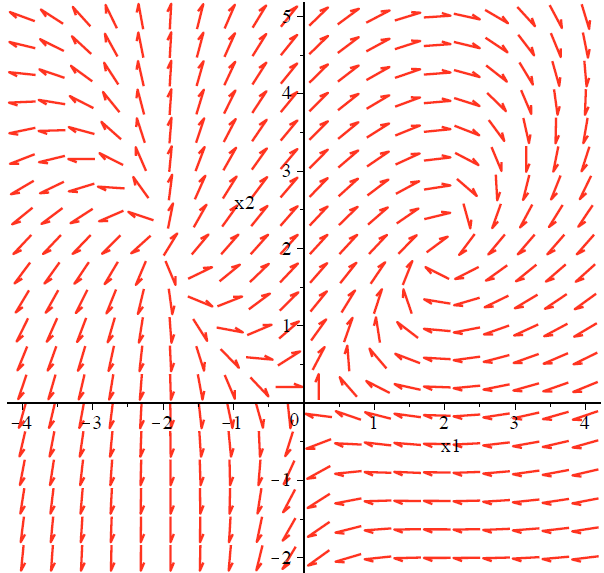
\includegraphics[width=0.9\textwidth]{images/Vektorfeld.png}
\end{minipage}
\begin{minipage}[h]{0.35\textwidth}
	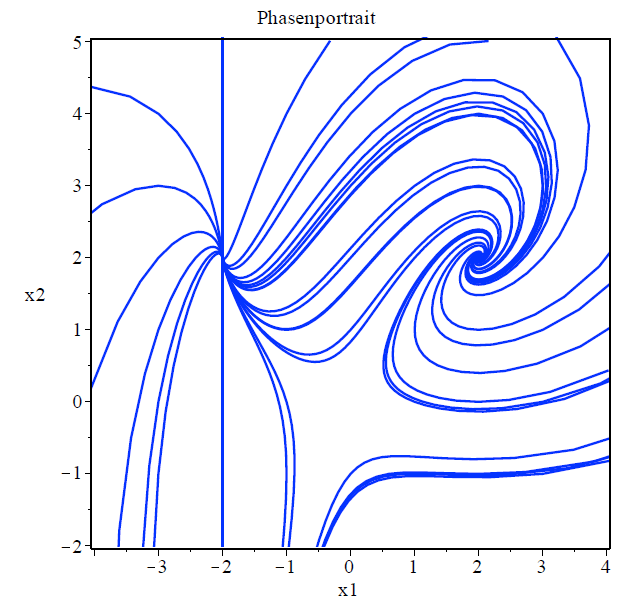
\includegraphics[width=1.0\textwidth]{images/Phasenportrait.png}
\end{minipage}